\newpage
\section{Développement}
\subsection{Création du moteur de jeu 3D}
    Pour composer les éléments du jeu et assurer une bonne qualité
    graphique et technique, le choix d'assembler le \emph{moteur de jeu 3D}
    \og \emph{RaptiquaX} \fg{} a été convenu. \emph{\Gls{SDL2}} permet un affichage dans un contexte
    \emph{\Gls{openGL}}, la librairie graphique la plus utilisée dans
    l'industrie du jeu vidéo avec la librairie \emph{Vulkan}
    \footnote{Vulkan \small{(anciennement \emph{OpenGL Next})}, a été
    développé par le groupe Khronos comme le successeur qui remplacera
    \Gls{openGL}.}.

    Pour permettre une composition modulable et accessible à tous, le modèle
    d'architecture de \emph{Godot}\footnote{Godot - 2014 - est un moteur de
    jeu libre multiplateforme proposant à la fois une interface en 2\up{e} et
    en 3\up{e} dimension.} a été utilisé comme référence, en raison de son
    potentiel\footnote{Godot a été très utilisé ces dernières années, même
    dans la réalisation de jeu dit AAA comme
    Sonic Colors Ultimate\cite{soniccoloru} }.

\subsubsection{Conception du moteur de rendu (OpenGL)}
    Un moteur de rendu graphique moderne sous \emph{\Gls{GLSL}} (ou ses
    alternatives\footnote{p. ex. HLSL sous Direct3D}) permet deux pipelines
    différentes et incompatibles\footnote{Depuis quelques années, la pipeline
    "Forward+" cherchant à mêler les deux par des méthodes avancées s'est
    popularisé.} \cite{iehl_deferred_vs_forward} :\\
    \begin{itemize}
        \item Le rendu différé qui permet d'appliquer le \gls{fragment shader}
        une seule fois par \gls{fragment} en utilisant plusieurs couches de
        rendu.
        \item Le rendu direct qui affiche immédiatement sans précalculer le
        \gls{GBuffer} ce qui peut s'avérer plus rapide selon le
        contexte.\\
    \end{itemize}

    Nous avons opté pour l'utilisation du rendu différé, car il permet de
    gérer plus facilement les effets de post-processing et d'optimiser le
    rendu de la lumière. De plus, il est plus adapté pour les scènes
    complexes avec de nombreux objets et lumières. (Pour aller plus loin sur
    le sujet, voir la section \ref{sec:deferred_rendering}).


    Le traitement de l'image est effectué majoritairement par le \gls{gpu},
    exploitant la stratégie inventée pas Silicon Graphics\cite{silicon_graphics}
    pour le traitement de l'image :\\
    \begin{itemize}
        \item Le \Gls{gpu} est divisé en plusieurs unités de calcul
        \item Chaque unité de calcul est responsable d'un aspect du rendu
        \item Les unités de calcul travaillent en parallèle pour traiter
        l'image rapidement
        \item La géométrie est transformée en primitives (triangles, lignes, points) par un programme appelé \emph{\gls{vertex shader}} (figure \ref{fig:sm64_wireframe})
        \item Les primitives sont ensuite \glslink{rasteriser}{rasterisées} pour créer des \glspl{fragment} (figure \ref{fig:sm64_result})\\
    \end{itemize}

    \begin{figure}[h]
        \begin{subfigure}{0.5\textwidth}
            \centering
            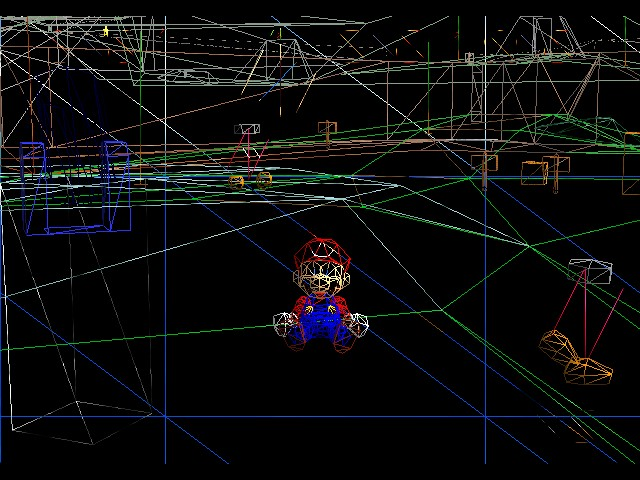
\includegraphics[width=0.8\textwidth]{images/m64wireframe.jpg}
            \caption{Super Mario 64 en mode fil de fer pour imager le \gls{vertex shader}}
            \label{fig:sm64_wireframe}
        \end{subfigure}
        \begin{subfigure}{0.5\textwidth}
            \centering
            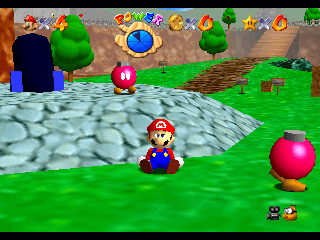
\includegraphics[width=0.8\textwidth]{images/m64result.png}
            \caption{Super Mario 64, après le passage par le \gls{fragment shader}}
            \label{fig:sm64_result}
        \end{subfigure}
        \caption{Exemple de rendu avec la stratégie de Silicon Graphics \cite{copetti_n64}}
        \label{fig:silicon_graphics_rendering}
    \end{figure}

    \newpage
    Enfin, le \gls{gpu} est de nouveau solicité pour le rendu de la scène
    finale, en utilisant les informations de la scène stockées dans le
    \gls{GBuffer} et en appliquant les effets de post-processing.
    Dans notre moteur, nous avons implémenté les techniques de rendu suivantes :
    \begin{multicols}{2}
    \begin{itemize}
        \item Le rendu différé
        \item Le rendu de la lumière en suivant le modèle de Phong 
        \item Le rendu des ombres en utilisant le \gls{shadow mapping}
        \item Le rendu de réflexions et de reflets en utilisant le \gls{ssr} (à but expérimental en utilisant le \gls{shader} de \emph{Imanol Fotia} \cite{imanolfotia})
        \item Le rendu d'occlusion ambiante en utilisant le \gls{ssao}
        \item Le rendu d'éblouissement en utilisant le \gls{bloom}
        \item L'anti-aliasing en utilisant le \gls{smaa}
    \end{itemize}
    \end{multicols}

    Une grande partie de ces techniques sont inspirées des travaux de Joey de Vries
    dans son site web LearnOpenGL \cite{learnopengl}, auquels nous avons
    ajouté des améliorations et des optimisations pour notre moteur grâce
    aux travaux de Adrian Courrèges sur DOOM 2016 \cite{courreges_doom2016}.
    \\ \\
    Pour un aperçu de la pipeline graphique de notre moteur, voir la section
    \ref{sec:graphics_pipeline}.

\subsubsection{Conception du moteur de physique}

    Le moteur de physique est responsable de la gestion des collisions et
    des interactions entre les objets de la scène. Il utilise un système de
    détection de collisions basé sur des formes géométriques simples, comme
    des sphères, des boîtes aux transformations non uniforme, des plans, etc.
    \\ \\
    La physique est ensuite calculée en utilisant une approche simplifiée des
    équations \emph{cinématiques} et des équations du \emph{principe fondamental de la dynamique}
    (\emph{deuxième loi de Newton}).

    \newpage

    Soit deux objets rigides, \( A \) et \( B \), se déplacent et entrent
    en collision. Voici comment nous calculons la réponse à la collision
    en utilisant les concepts de base de la physique des corps rigides.

    \begin{multicols}{2}

        \paragraph{Norme de la collision}
        La norme de la collision entre les deux corps est donnée par un vecteur
        normal à la surface de collision. Si les corps ont une normale de
        collision définie, cette norme est utilisée dans les calculs suivants.
    
        \nomenclature{$\mathbf{n}$}{Vecteur normal à la surface de collision}
        \nomenclature{$\mathbf{\lambda}_A$}{Normale de l'objet $A$}
        \nomenclature{$\mathbf{\lambda}_B$}{Normale de l'objet $B$}
        
        \begin{equation}
        \mathbf{n} = \mathbf{\lambda}_A \cdot \mathbf{\lambda}_B
        \end{equation}
    
        \paragraph{Vitesse relative}
        La vitesse relative des deux objets rigides \( A \) et \( B \) est calculée
        comme la différence entre leurs vitesses respectives :
    
        \nomenclature{$\mathbf{v}_{\text{relative}}$}{Vitesse relative entre deux objets}
        \nomenclature{$\mathbf{v}_A$}{Vitesse de l'objet $A$}
        \nomenclature{$\mathbf{v}_B$}{Vitesse de l'objet $B$}
        
        \begin{equation}
        \mathbf{v}_{\text{relative}} = \mathbf{v}_B - \mathbf{v}_A
        \end{equation}
    
        \paragraph{Vitesse relative selon la direction normale}
        \nomenclature{$v_{\text{normal}}$}{Vitesse relative projetée sur la normale de collision}
        
        \begin{equation}
        v_{\text{normal}} = \mathbf{v}_{\text{relative}} \cdot \mathbf{n}
        \end{equation}
    
        \paragraph{Coefficient de restitution (élasticité de la collision)}
        \nomenclature{$e$}{Coefficient de restitution}
        
        \begin{equation}
        e = 0.02
        \end{equation}
    
        \columnbreak
    
        \paragraph{Calcul de l'impulsion}
        \nomenclature{$I_{scalaire}$}{Quantité scalaire représentant l'impulsion échangée}
        \nomenclature{$m_A$}{Masse de l'objet $A$}
        \nomenclature{$m_B$}{Masse de l'objet $B$}
        
        \begin{equation}
        I_{scalaire} = \frac{(1 + e) \cdot v_{\text{normal}}}{m_A^{-1} + m_B^{-1}}
        \end{equation}
    
        \paragraph{Calcul du vecteur d'impulsion}
        \nomenclature{$\mathbf{I}$}{Vecteur d'impulsion appliqué pendant la collision}
        
        \begin{equation}
        \mathbf{I} = I_{scalaire} \cdot \mathbf{n}
        \end{equation}
    
        \paragraph{Application de l'impulsion et du couple}
        \nomenclature{$\mathbf{r}_A$}{Vecteur du centre de masse de $A$ au point d’impact}
        \nomenclature{$\mathbf{r}_B$}{Vecteur du centre de masse de $B$ au point d’impact}
        \nomenclature{$\mathbf{C}_A$}{Centre de masse de $A$}
        \nomenclature{$\mathbf{C}_B$}{Centre de masse de $B$}
        \nomenclature{$\mathbf{P}_{\text{impact}}$}{Point d’impact}
        
        \begin{equation}
        \mathbf{r}_A = \mathbf{P}_{\text{impact}} - \mathbf{C}_A
        \end{equation}
        \begin{equation}
        \mathbf{r}_B = \mathbf{P}_{\text{impact}} - \mathbf{C}_B
        \end{equation}
        \begin{equation}
        \text{Couple sur A} = \mathbf{r}_A \times \mathbf{I}
        \end{equation}
        \begin{equation}
        \text{Couple sur B} = \mathbf{r}_B \times \mathbf{I}
        \end{equation}
    
        \paragraph{Application de l'impulsion}
        \nomenclature{$\mathbf{v}_A'$}{Nouvelle vitesse de l’objet $A$}
        \nomenclature{$\mathbf{v}_B'$}{Nouvelle vitesse de l’objet $B$}
        
        \begin{equation}
        \mathbf{v}_A' = \mathbf{v}_A + \mathbf{I} \cdot m_A^{-1}
        \end{equation}
        \begin{equation}
        \mathbf{v}_B' = \mathbf{v}_B - \mathbf{I} \cdot m_B^{-1}
        \end{equation}
    
        \paragraph{Correction de la pénétration}
        \nomenclature{$\delta$}{Profondeur de pénétration}
        \nomenclature{$\mathbf{C}$}{Correction appliquée pour compenser la pénétration}
        \nomenclature{$\mathbf{P}_A$}{Position initiale de l'objet $A$}
        \nomenclature{$\mathbf{P}_B$}{Position initiale de l'objet $B$}
        \nomenclature{$\mathbf{P}_A'$}{Nouvelle position de l'objet $A$}
        \nomenclature{$\mathbf{P}_B'$}{Nouvelle position de l'objet $B$}
        
        \[
        \mathbf{C} = \delta \cdot \mathbf{n}
        \]
        \begin{equation}
        \mathbf{P}_A' = \mathbf{P}_A - \mathbf{C}
        \end{equation}
        \begin{equation}
        \mathbf{P}_B' = \mathbf{P}_B + \mathbf{C}
        \end{equation}
    
        \paragraph{Calcul du couple et de l'inertie}
        \nomenclature{$\mathbf{I}_{\text{locale}}$}{Matrice d’inertie locale}
        \nomenclature{$w$}{Largeur de l'objet}
        \nomenclature{$h$}{Hauteur de l'objet}
        \nomenclature{$d$}{Profondeur de l'objet}
    
        \begin{equation}
        \mathbf{I}_{\text{locale}} = \frac{m}{12} \begin{bmatrix} h^2 + d^2 & 0 & 0 \\ 0 & w^2 + d^2 & 0 \\ 0 & 0 & w^2 + h^2 \end{bmatrix}
        \end{equation}
    
        \paragraph{Accélération angulaire}
        \nomenclature{$\mathbf{\alpha}$}{Accélération angulaire}
        \nomenclature{$\mathbf{T}$}{Couple appliqué}
        \nomenclature{$\mathbf{I}^{-1}$}{Inverse de la matrice d’inertie}
        
        \begin{equation}
        \mathbf{\alpha} = \mathbf{I}^{-1} \cdot \mathbf{T}
        \end{equation}
    
    \end{multicols}

\subsubsection{Conception de l'arbre de données}

    Dans notre moteur, nous avons choisi d'utiliser un arbre de données
    pour représenter la scène 3D. Cet arbre est composé de n\oe{}uds, où
    chaque n\oe{}ud représente un objet de la scène. Chaque n\oe{}ud
    contient des informations sur la position, la rotation et l'échelle de
    l'objet, ainsi que des références vers ses enfants et son père.
    Cela permet de créer une hiérarchie d'objets, où chaque objet peut
    être transformé indépendamment tout en étant affecté par les
    transformations de ses parents.
    \\ \\
    Ce modèle d'arbre de données est inspiré du moteur de jeu Godot, qui
    utilise également un arbre de n\oe{}uds pour représenter une scène.
    \\ \\
    Les n\oe{}uds de l'arbre sont génériques, ce qui garantit un stockage
    efficace des données et une gestion facile des objets de la scène (figure \ref{fig:node_structure}).

    \begin{figure}[h]
        \centering
        \includesvg[width=\linewidth]{images/node.svg}
        \emph{La structure présentée ici est une simplification de la structure utilisée dans notre moteur de jeu.}
        \caption{Structure d'un noeud générique}
        \label{fig:node_structure}
    \end{figure}

    Vous pouvez vous référer à la table \ref{tab:raptiquax_nodes} pour découvrir
    les différents types de n\oe{}uds que nous avons implémentés dans notre
    moteur de jeu. Chaque n\oe{}ud est responsable d'un aspect spécifique de
    la scène, ce qui permet de créer un tout cohérent et fluide.


\subsubsection{Conception des classes et héritage}

    Pour assurer une bonne organisation du code et une gestion efficace
    des objets de la scène, nous avons utilisé un système de classes capable
    de gérer l'héritage.
    \\ \\
    Le code source du moteur est précompilé par un outil développé par nos
    soins, qui permet de générer un code source en C à partir d'un fichier
    classe inspiré de la syntaxe de \emph{C++}. Les classes ainsi générées
    sont ensuites liées entre elles par un header de liaison, lui aussi
    généré par l'outil. Cela permet de créer un code source propre et
    facilement lisible, tout en assurant une bonne gestion de la mémoire et des
    performances.
    \\ \\
    Un exemple des classes utilisées par l'outil de précompilation est
    présenté dans le listing \ref{lst:class_template}.
    \\ \\
    Le code source généré utilise les arguments variadiques et prend en charge
    les promotions automatiques des types.
\subsubsection{Conception des entrées sorties}

    Le moteur prend en charge les entrées/sorties de sorte à permettre
    aux développeurs de créer des jeux en utilisant des fichiers de
    ressources sans avoir à se soucier de l'implémentation ou de la gestion
    de la mémoire et des performances.
\paragraph{Chargement des ressources}

    Les ressources du moteurs sont chargées à l'aide de diverses
    fonctions d'entrée/sortie, qui permettent de charger des fichiers
    de différents formats. Voici une liste non exhaustive des formats
    de fichiers pris en charge par le moteur :\\
    \begin{itemize}
        \item \textbf{OBJ} : format de fichier 3D utilisé pour stocker
        des modèles 3D. Il est simple et largement utilisé dans
        l'industrie du jeu vidéo. \cite{obj_format}
        \item \textbf{PNG} : format de fichier image utilisé pour stocker
        des textures.
        \item \textbf{JPG} : format de fichier image compressé utilisé pour stocker
        des textures.
        \item \textbf{WAV} : format de fichier audio brut utilisé pour stocker
        des sons.
        \item \textbf{OGG} : format de fichier audio compressé utilisé généralement pour
        stocker des sons.
        \item \textbf{MP3} : format de fichier audio compressé utilisé généralement pour
        stocker des musiques.
        \item \textbf{SCENE} : format de fichier propriétaire utilisé pour
        stocker des scènes 3D.
        \item \textbf{FS} : format de fichier shader utilisé pour stocker
        des shaders de fragment. \cite{glsl}
        \item \textbf{VS} : format de fichier shader utilisé pour stocker
        des shaders de vertex. \cite{glsl}\\
    \end{itemize}
    
    Les ressources sont stockées en cache pour éviter de les recharger
    plusieurs fois. Le moteur utilise un système de gestion de
    ressources qui permet de charger et de décharger les ressources
    du cache sur demande. Cela permet de réduire la consommation de mémoire et
    d'optimiser les performances du moteur.
\paragraph{Communication en réseau (SocketIO)}

    Le moteur permet en outre de gérer la communication en réseau entre
    des clients et un serveur en multithreads. Pour cela, nous avons utilisé
    la librairie \emph{Socket} en C, qui permet de gérer la communication en
    temps réel entre le serveur et les clients.
    Nous avons implémenté un serveur Socket qui gère les connexions des
    clients et les messages échangés entre eux. Le serveur est capable de
    gérer plusieurs clients en même temps et de leur envoyer des messages
    en temps réel. Il est également capable de gérer les connexions et
    déconnexions des clients, ainsi que les erreurs de communication.
    Le serveur de démonstration que nous avons mis en place est capable de
    gérer une dizaine de commandes différentes (table \ref{tab:raptiquax_requests}).
    \\ \\
    Comme preuve de concept, nous avons mis en place un serveur pour \og \emph{FPS Chess} \fg{}, un
    mini-jeu fps multijoueur qui gère plusieurs parties de deux joueurs en même temps.

\subsection{Création des ressources}
\subsubsection{Conception du modèle 3d et des textures}
La map du jeu, représentant le bâtiment Claude Chappe et ses
environs, a été créée en plusieurs étapes via Blender : \\ \\
\textbf{- Modélisation 3D des modèles :} \\
\\
On utilise des objets préfabriqués de Blender, modifiables
grâce à divers outils pour obtenir les formes désirées (ex :
transformation d'un cube en mur ou en porte comme on le voit
figure ~\ref{fig:cube-base} et ~\ref{fig:cube-modif}). Nous
avons d'abord modélisé la structure de base du bâtiment, puis
ajouté des éléments exclusifs au jeu, comme des trous dans le
sol et les murs pour un parcours de poursuite, ainsi que trois
salles secrètes avec des ordinateurs pour les mini-jeux.\\

\textbf{- Normals :} \\\\
Les normales définissent l'orientation des faces des objets et
influencent l'effet de la lumière. Bien que généralement correctes
par défaut, il est parfois nécessaire de les ajuster pour éviter
des erreurs d'affichage. \\

\textbf{- Texturage :} \\ \\
Une fois les objets modélisés, ils sont texturés en utilisant des
textures d’image ou des couleurs unies, compatibles avec le
moteur 3D. Par exemple, une porte est texturée en rouge uni,
tandis que les murs utilisent une texture image de plastique
gris/blanc.\\

\textbf{- Séparation des zones :} \\

Les objets sont regroupés en "collections" selon leur emplacement
(amphithéâtre, couloirs, salles de classe, etc.), ce qui facilite
leur exportation en fichiers .obj distincts et optimise le
chargement des ressources dans le moteur.\\

\textbf{- Optimisation des modèles et textures :} \\

Les erreurs de modélisation sont corrigées pour garantir une
bonne intégration. Les UV Maps des textures sont ajustées pour
assurer un affichage correct après l'exportation.\\

\textbf{- Exportation :} \\

Les objets d’une zone sont fusionnés (JOIN) pour simplifier
l’importation dans le moteur (un seul objet au lieu de plusieurs
centaines). On les exporte ensuite en .obj et .mtl (textures), en
veillant à inclure toutes les images de textures nécessaires.

\begin{figure}
    \centering
    \begin{minipage}{0.49\linewidth}
        \centering
        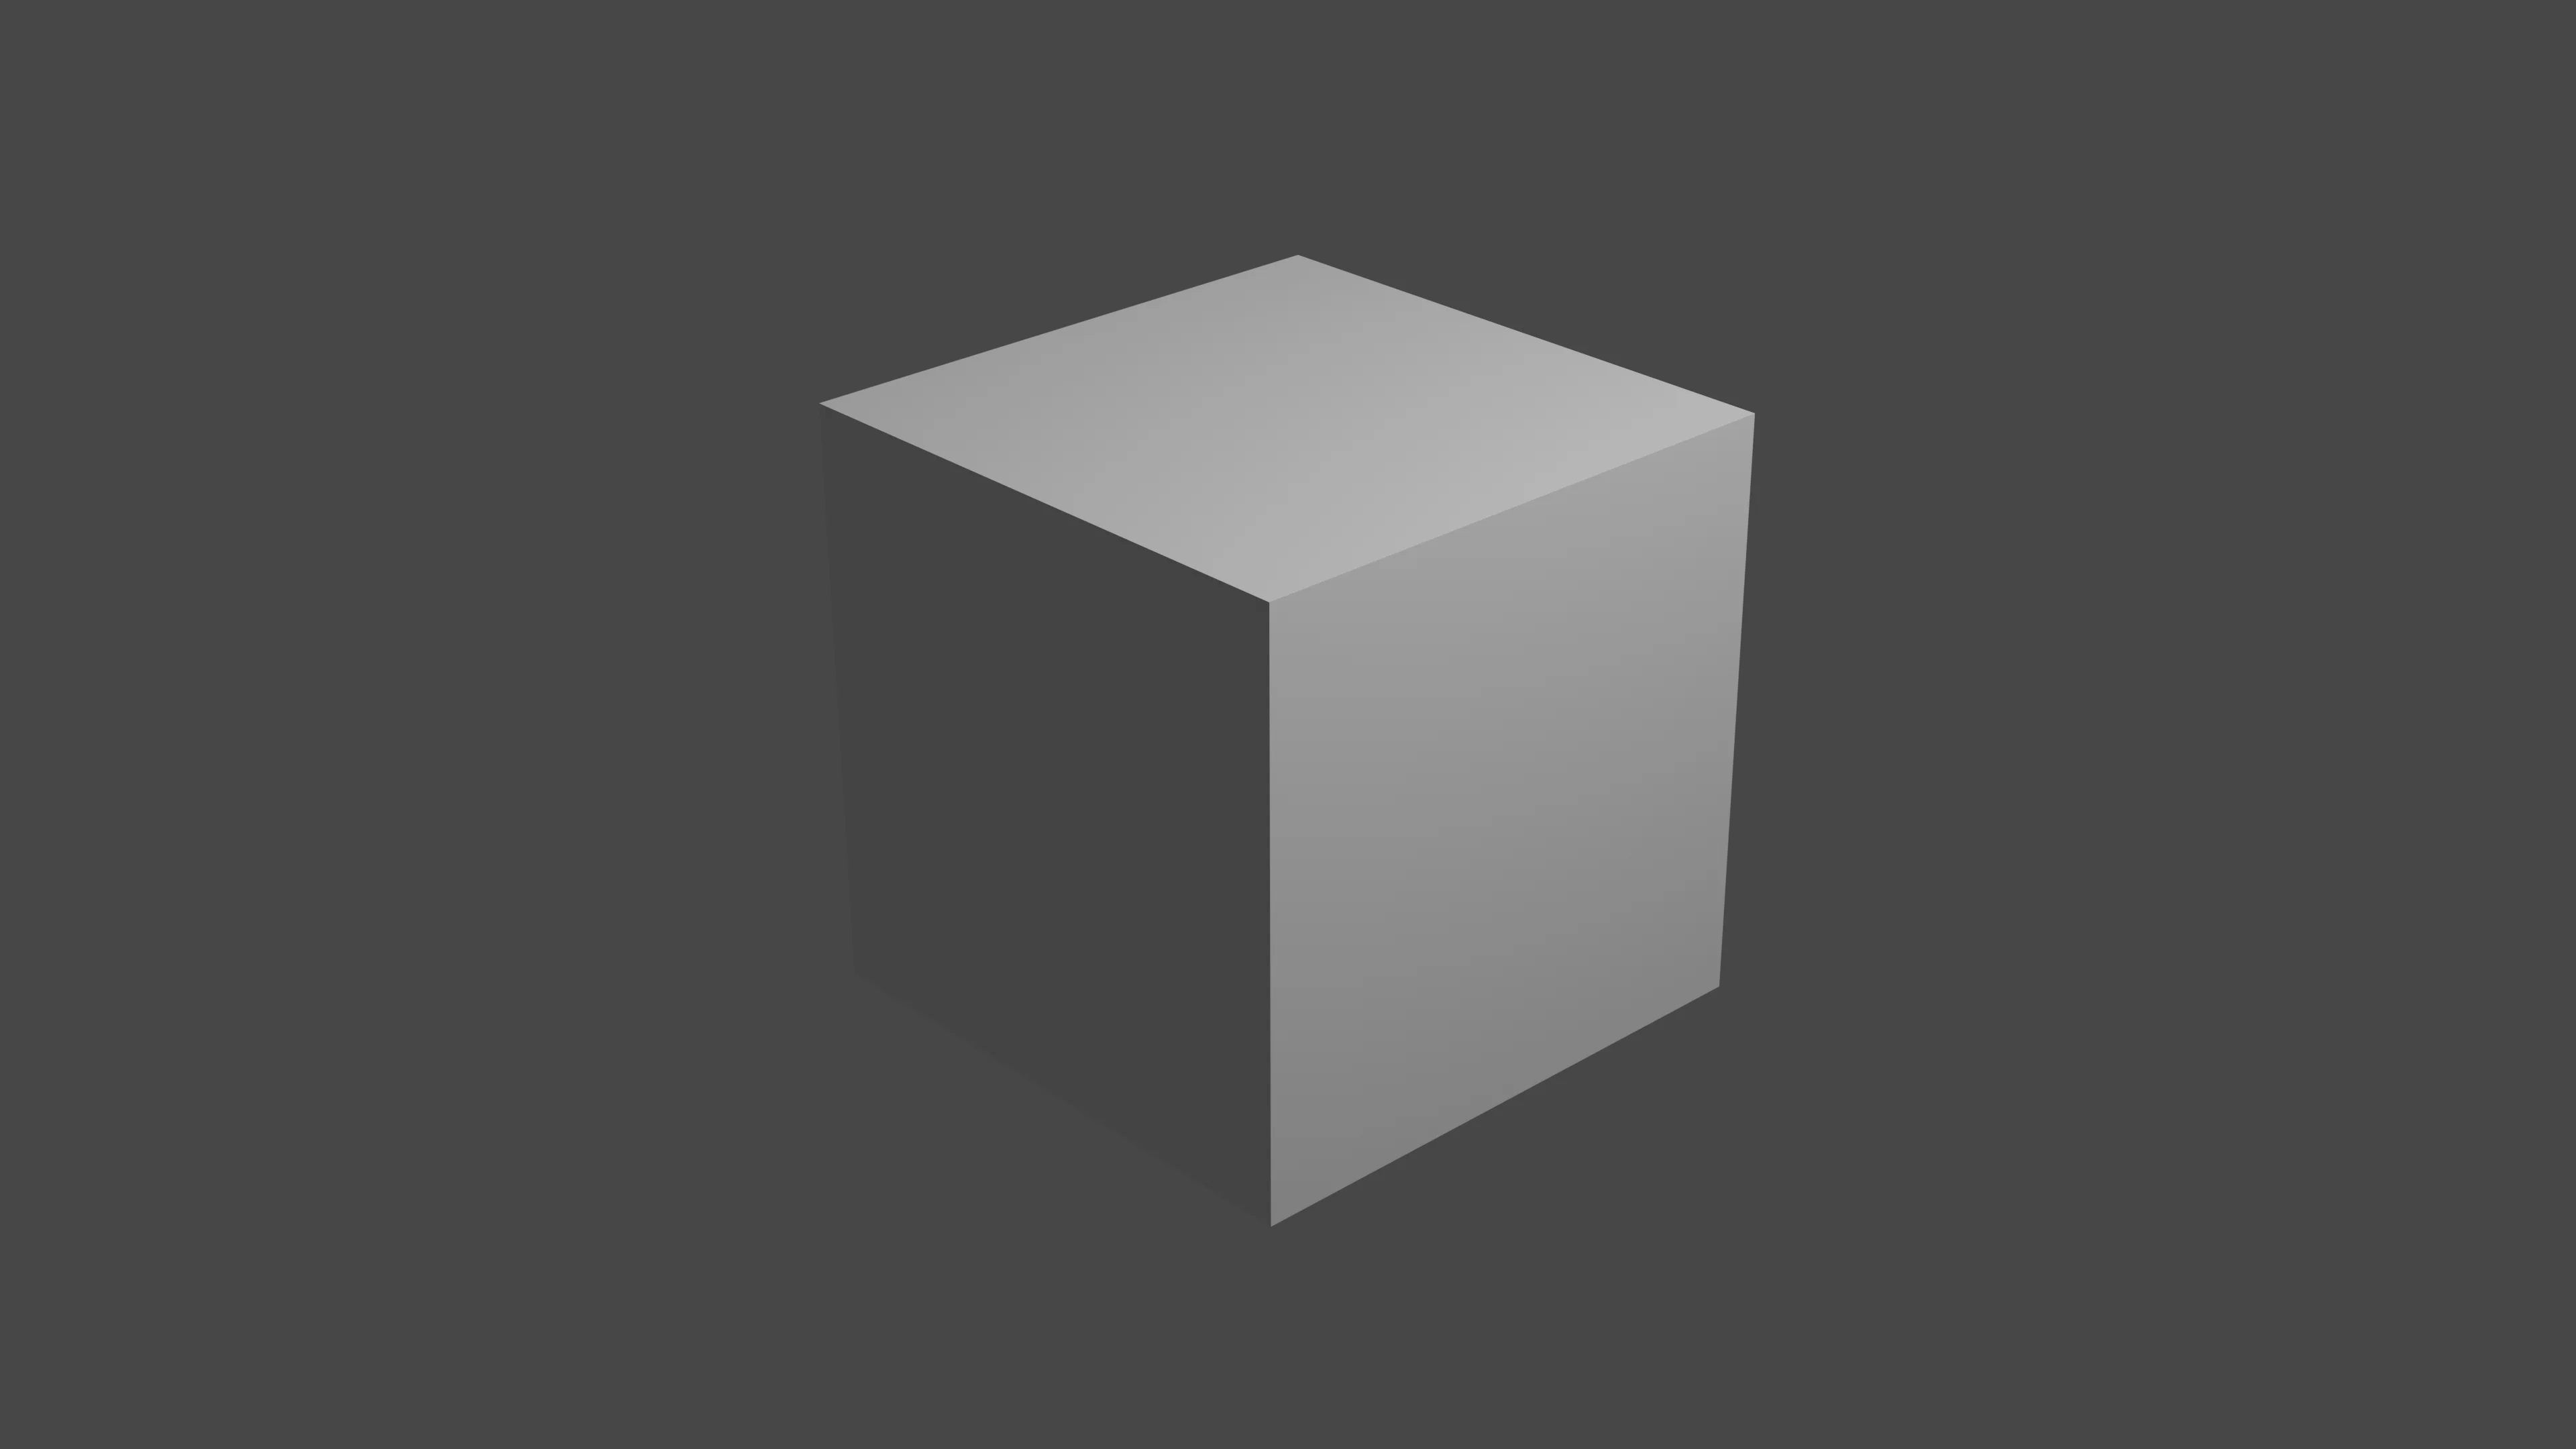
\includegraphics[width=\linewidth]{images/base_cube.png}
        \caption{Cube de base Blender}
        \label{fig:cube-base}
    \end{minipage}
    \hfill
    \begin{minipage}{0.49\linewidth}
        \centering
        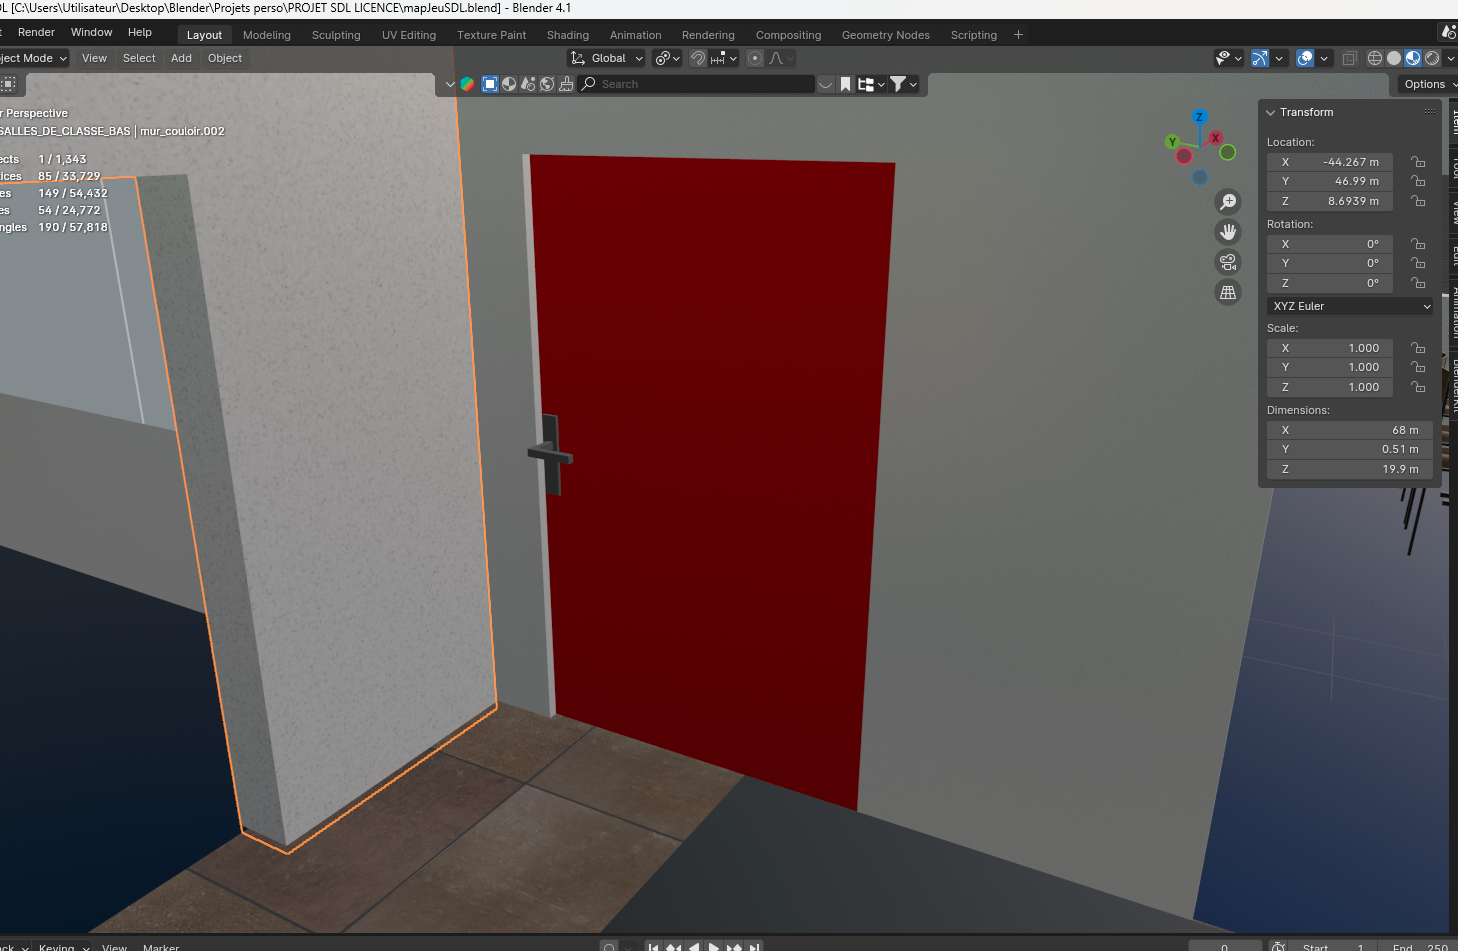
\includegraphics[width=\linewidth]{images/cubemodif.png}
        \caption{Cubes modifiés en divers objets}
        \label{fig:cube-modif}
    \end{minipage}
\end{figure}
\subsubsection{Conception des musiques et effets sonores}

Les musiques et les effets sonores sont tous les deux composés
sur le logiciel FL Studio.\\\\
\textbf{- Conception des musiques :}\\\\
À partir de sons déjà existants (libres de droits), on les
utilise en les modifiant (ou non), pour en faire des mélodies
(à l'aide d'un clavier synthétiseur), des boucles de divers instruments,
bref créer une musique.\\\\
\textbf{- Conception des effets sonores :}\\\\
Pour les effets sonores, on utilise à nouveau des sons déjà
existants, évidemment sans faire des mélodies cette fois. On les
modifie à travers divers plugins du logiciel (pitch grave/aigu,
réverbération, etc.).\\
Vous trouverez en annexe un exemple de composition musicale (voir figure \ref{fig:flstudio.png}).
\subsection{Gestion des scènes}
\subsubsection{Gestion des objets}

Les objets sont des entités gérées par des scripts importés dans les scènes du
moteur 3D.
\\ \\
Les scripts sont écrits en C et sont chargés par le moteur 3D au moment de
l'importation de la scène. Ils sont ensuite exécutés par le moteur 3D lors de
la boucle de jeu à des instants clés.
\\ \\
On peut ainsi définir des comportements spécifiques pour l'initialisation
des objets, leur mise à jour et lors de la réception de signaux.
\\ \\
Les interactions entre les objets et l'environnement sont gérées par ces
signaux qui sont émis notamment lorsque les objets entrent en collision avec
d'autres objets, mais il est possible de paramétrer divers signaux personnalisés.

\paragraph{Mini-jeux}
Dans le cadre de Chapper's Fallout, les mini-jeux en 2D sont conçus pour être totalement intégrés au sein d’un environnement homogène. Chaque mini-jeu débute 
par l’activation d’une fenêtre qui simule le démarrage d’un ordinateur. Cette fenêtre, gérée par un système de fenêtrage complet, initialise automatiquement 
l’affichage du bureau virtuel et coordonne le déroulement des scènes à l’aide d’un gestionnaire d’événements centralisé.
\\ \\
Le premier mini-jeu, par exemple, présente un bureau sur lequel se trouvent des icônes décoratives. Le cœur du gameplay repose sur l’apparition de 
notifications qui indiquent la prochaine mission. Ici, le joueur reçoit un message de Souleymane lui demandant de le rejoindre pour un TP dans le bâtiment CC. 
Une fois le message accepté via une interaction clavier ou souris, la fenêtre signale la fin du mini-jeu et permet le retour fluide dans le monde 3D.
\\ \\
Le second mini-jeu suit une logique similaire : l’ordinateur se lance dans une nouvelle fenêtre affichant le bureau, puis, en cliquant sur une icône spécifique, 
le joueur accède à un jeu en 2D. Ce dernier consiste à esquiver des objets projetés depuis les bords de la fenêtre. Une fois l’épreuve terminée, le joueur peut 
ouvrir un fichier interactif, conçu pour afficher des lignes de code de l’IA, et tenter de modifier ces paramètres pour réparer le système, même si l’issue n’est 
pas toujours favorable.
\\ \\
Le troisième mini-jeu reprend le même mécanisme de lancement d’ordinateur. Après l’affichage du bureau, le joueur est amené à réaliser un jeu de décodage simple, 
où il doit décrypter une série de symboles. La réussite de cette épreuve permet d’accéder à un fichier de nettoyage, indispensable pour poursuivre la réparation 
de l’IA.
\\ \\
Au niveau du code, la gestion des événements est assurée par une boucle principale qui interroge SDL afin de capter en temps réel les entrées utilisateur (clics, 
déplacements de souris, frappes clavier). Chaque mini-jeu possède ainsi son propre « event manager » qui orchestre les transitions entre les différentes scènes. 
Par ailleurs, le système de gestion de fenêtres permet de créer, mettre à jour et détruire les fenêtres de jeu en synchronisation avec ces événements, assurant 
ainsi une expérience utilisateur fluide et réactive.
\\ \\
Les structures de données, notamment celles dédiées aux éléments du bureau et aux textures animées, jouent un rôle crucial dans l’animation et 
l’affichage des éléments graphiques. Par exemple, la fonction de mise à jour des textures incrémente le compteur de frames pour afficher la portion adéquate d’un 
spritesheet, garantissant une animation cohérente et dynamique. Ce modèle a d’ailleurs été pensé pour être facilement extensible, afin d’ajouter de nouvelles 
interactions ou de modifier l’ordre des scènes sans perturber le fonctionnement global du système.
\\ \\
Dans l’ensemble, ce design modulaire basé sur le système de fenêtrage intégré, couplé à une gestion des événements et une architecture orientée scène, permet de 
créer des mini-jeux diversifiés et immersifs, renforçant ainsi l’expérience globale du joueur dans l’univers de Chapper's Fallout.

\subsubsection{Gestion des PNJ (personnages non joueurs)}

Les PNJ sont des entités qui se déplacent dans la scène. Ils sont gérés par le moteur
3D et sont placés dans la scène via l'éditeur de niveau. Leurs comportements sont
défini par des scripts qui sont exécutés par le moteur et utilisent le principe
de la machine à état.\\

Pour rendre les PNJ plus réalistes, nous avons implémenté un système de chemins
de navigation. Ce système permet aux PNJ de se déplacer le long d'un chemin prédéfini
dans la scène. Les chemins sont définis par des points de contrôle placés dans
la scène. Le moteur 3D utilise ces points de contrôle pour calculer la trajectoire
des PNJ et les faire se déplacer le long de cette trajectoire.

\subsubsection{Placement des collisions}
Une fois que le modèle est affiché et que tous les obstacles et éléments de
décors sont placés, il faut qu'on puisse intéragir avec eux.
\\ \\
Pour éviter de passer à travers les murs il faut detecter quand le joueur
est à la même position que le mur en question.
\\ \\
On a choisi d'abord d'afficher le modèle 3D, ensuite grâce à l'éditeur on
place des "boites" de collisions. En jeu ces boîte seront invisible, mais
infranchissable, ça permet de ne pas traverser les obstacles.
\\ \\
Par exemple on modelise une table avec le moteur 3D. Dans l'éditeur on rajoute
manuellement une "boite" de collisions à l'emplacement de la table, on cherche
à épouser la forme de la table. En jeu on verra que la table, et on ne pourra
pas la traverser, on peut même monter dessus etc.
\\ \\
Sur la figure \ref{fig:fig2} montre les différents types de "boîtes" On voit qu'on dessine
chaque éléments avec des boîtes.



\begin{figure}[H]
    \centering
    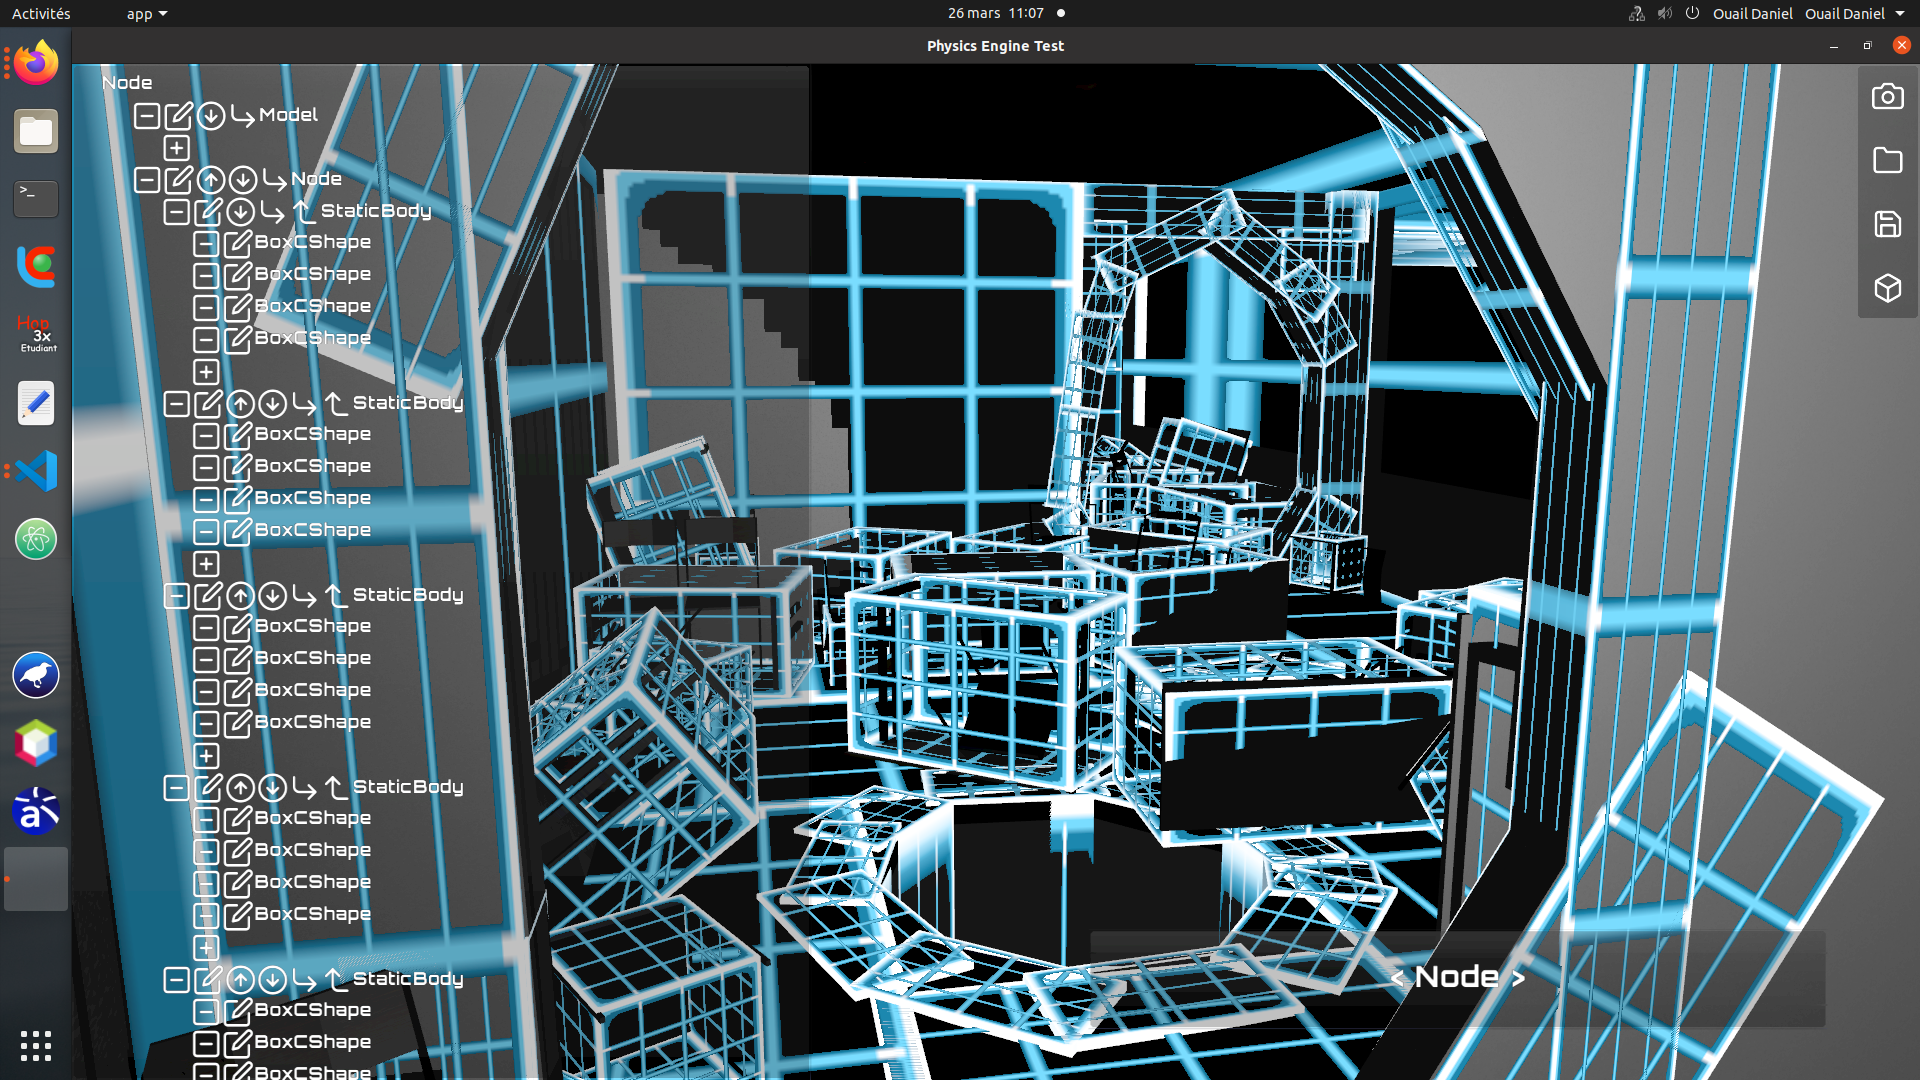
\includegraphics[width=1\linewidth]{images/screenshot_editeur.png}
    \caption{Capture d'écran de l'éditeur de niveau}
    \label{fig:fig2}
\end{figure}

Les coordonnées de chaque boîtes de collisions sont enregistrées avec l'éditeur
dans un fichier .scene, ce fichier sera lu au moment de l'execution pour
charger le modèle et les collisions.



\newpage